%%%%% !TEX root=template.tex
%%%%%%%%%%%%%%%%%%%%%%%%%%%%%%%%%%%%%%%%%%%%%%%%%%%%%%%%%%%%%%%%%%%%%%%%
%% template.tex
%% NOVA thesis main document file
%%
%% This work is licensed under the
%% The LaTeX project public license (LPPL), version 1.3c
%% To view a copy of this license, visit
%% https://www.latex-project.org/lppl/lppl-1-3c/
%%
%% Version 2025-05-25 [7.3.7]
%% Departamento de Informática (www.di.fct.unl.pt)
%% Faculdade de Ciências e Tecnologia (www.fct.unl.pt)
%% Universidade NOVA de Lisboa (www.unl.pt)
%%
%% BUGS and SUGGESTIONS: please submit an issue at the project web page
%%      at: https://github.com/joaomlourenco/novathesis/
%%
%% HELP: please DO NOT SEND ME EMAILS about LaTeX or the NOVAthesis template
%%       please ask for help at GitHub Discussions page at
%%          https://github.com/joaomlourenco/novathesis/discussions
%%      or at the NOVAthesis facebook group at
%%          https://www.facebook.com/groups/novathesis
%%      or in the subreddit r/novathesis
%%          https://www.reddit.com/r/novathesis/
%%
%% AUTHOR @github:
%%      - joaomlourenco
%%
%% CONTRIBUTORS @github:
%%      https://github.com/joaomlourenco/novathesis/wiki#help-with-the-project-patches-and-new-features
%%
%% DONATIONS:
%%      If you think this template really helped you while writing your thesis, then
%%          1. Go to the project web page and giv it a star (on the top-right)
%%          2. Make a small donation using the URL below
%%                    https://www.paypal.com/donate/?hosted_button_id=8WA8FRVMB78W8
%%             We will keep a list thanking to all the identified donors that identify
%%             themselves in the “Add special instructions to the seller:” box.
%%
%% CITATION:
%%      If you use this template, please be kind and \cite{novathesis-manual} somewhere in your document.
%%%%%%%%%%%%%%%%%%%%%%%%%%%%%%%%%%%%%%%%%%%%%%%%%%%%%%%%%%%%%%%%%%%%%













%%%%%%%%%%%%%%%%%%%%%%%%%%%%%%%%%%%%%%%%%%%%%%%%%%%%%%%%%%%%%%%%%%%%%
% PLEASE DO NOT CHANGE THIS FILE
% ALL THE CUSTOMIZATION WAS MOVED TO THE files in the ”Config” FOLDER
%%%%%%%%%%%%%%%%%%%%%%%%%%%%%%%%%%%%%%%%%%%%%%%%%%%%%%%%%%%%%%%%%%%%%




















%%============================================================
%% BLACK VOID AHEAD!  DO NOT TRESPASS!
%%============================================================










%%============================================================
%% YOU'VE BEEN WARNED.  GO BACK TO SAFE GROUND.  NOW!!!
%%============================================================










%%============================================================
%%  DO NOT GO BEYOND THIS POINT!
%%  IF YOU DO… YOU DESERVE WHATEVER HAPPENS AFTERWARDS!
%%============================================================





%%------------------------------------------------------------
%% The novathesis class is based in “memoir”.  To set memoir
%%  options, edit “Config/0_memoir.tex”.
\RequirePackage{NOVAthesisFiles/fix-profiling}
\texprof{\benchmarktic}
\documentclass{novathesis}


%============================================================
%  MEMOIR CUSTOMIZATION
%      Please open and edit the appropriate
%       configuration file “Config/0_memoir.tex”
%============================================================

%============================================================
%  TEMPLATE CUSTOMIZATION / OPTIONS (document type, university, school, etc)
%      Please open and edit the appropriate
%       configuration file “Config/1_novathesis.tex”
%============================================================

%============================================================
% BIBLATEX CUSTOMIZATION (citation and bibliography styles)
%      Please open and edit the appropriate
%       configuration file “Config/2_biblatex.tex”
%============================================================

%============================================================
%  COVER CUSTOMIZATION (title, author, etc)
%   Please open and edit the appropriate
%       configuration file “Config/3_cover.tex”
%============================================================

%============================================================
%  THESIS/DISSERTATION FILES
%   Please open and edit the appropriate
%       configuration file “Config/4_files.tex”
%============================================================

%============================================================
%  PERSONAL (YOUR) CUSTOMIZATION
%   Please open and edit the appropriate
%       configuration file “Config/5_packages.tex”
%============================================================

%============================================================
%  WHICH LIST_OF TO PRINT
%   Please open and edit the appropriate
%       configuration file “Config/6_list_of.tex”
%============================================================

%============================================================
% SPECIAL UNIVERSITY/SCHOOL CUSTOMIZATION
%      Please open and edit the appropriate
%       configuration file “Config/9_UNIVERSITY.tex”
%============================================================


















%%============================================================
%% HAVE I NOT TOLD YOU TO NOT EDIT/CHANGE THIS FILE???  YES I DID!!!
%%============================================================

%%------------------------------------------------------------
\begin{document}          % Beginning of document
\texprof{\benchmarktoc}
\texprof{\typeout{TIME class loading=\the\pdfelapsedtime}}
%%------------------------------------------------------------
%% Print covers
\texprof{\benchmarktic}
\ntthesisfrontmatter      % Before the main text (TOC, etc) — Roman page numbering
\ntprint{covers}          % The cover page
\texprof{\benchmarktoc}
\texprof{\typeout{TIME process covers=\the\pdfelapsedtime}}

\thispagestyle{empty}
\begin{tikzpicture}[remember picture,overlay]
    \node (fondo) [rectangle]
    at (current page.center)
        {\parbox[b][\paperheight]{\paperwidth}{
        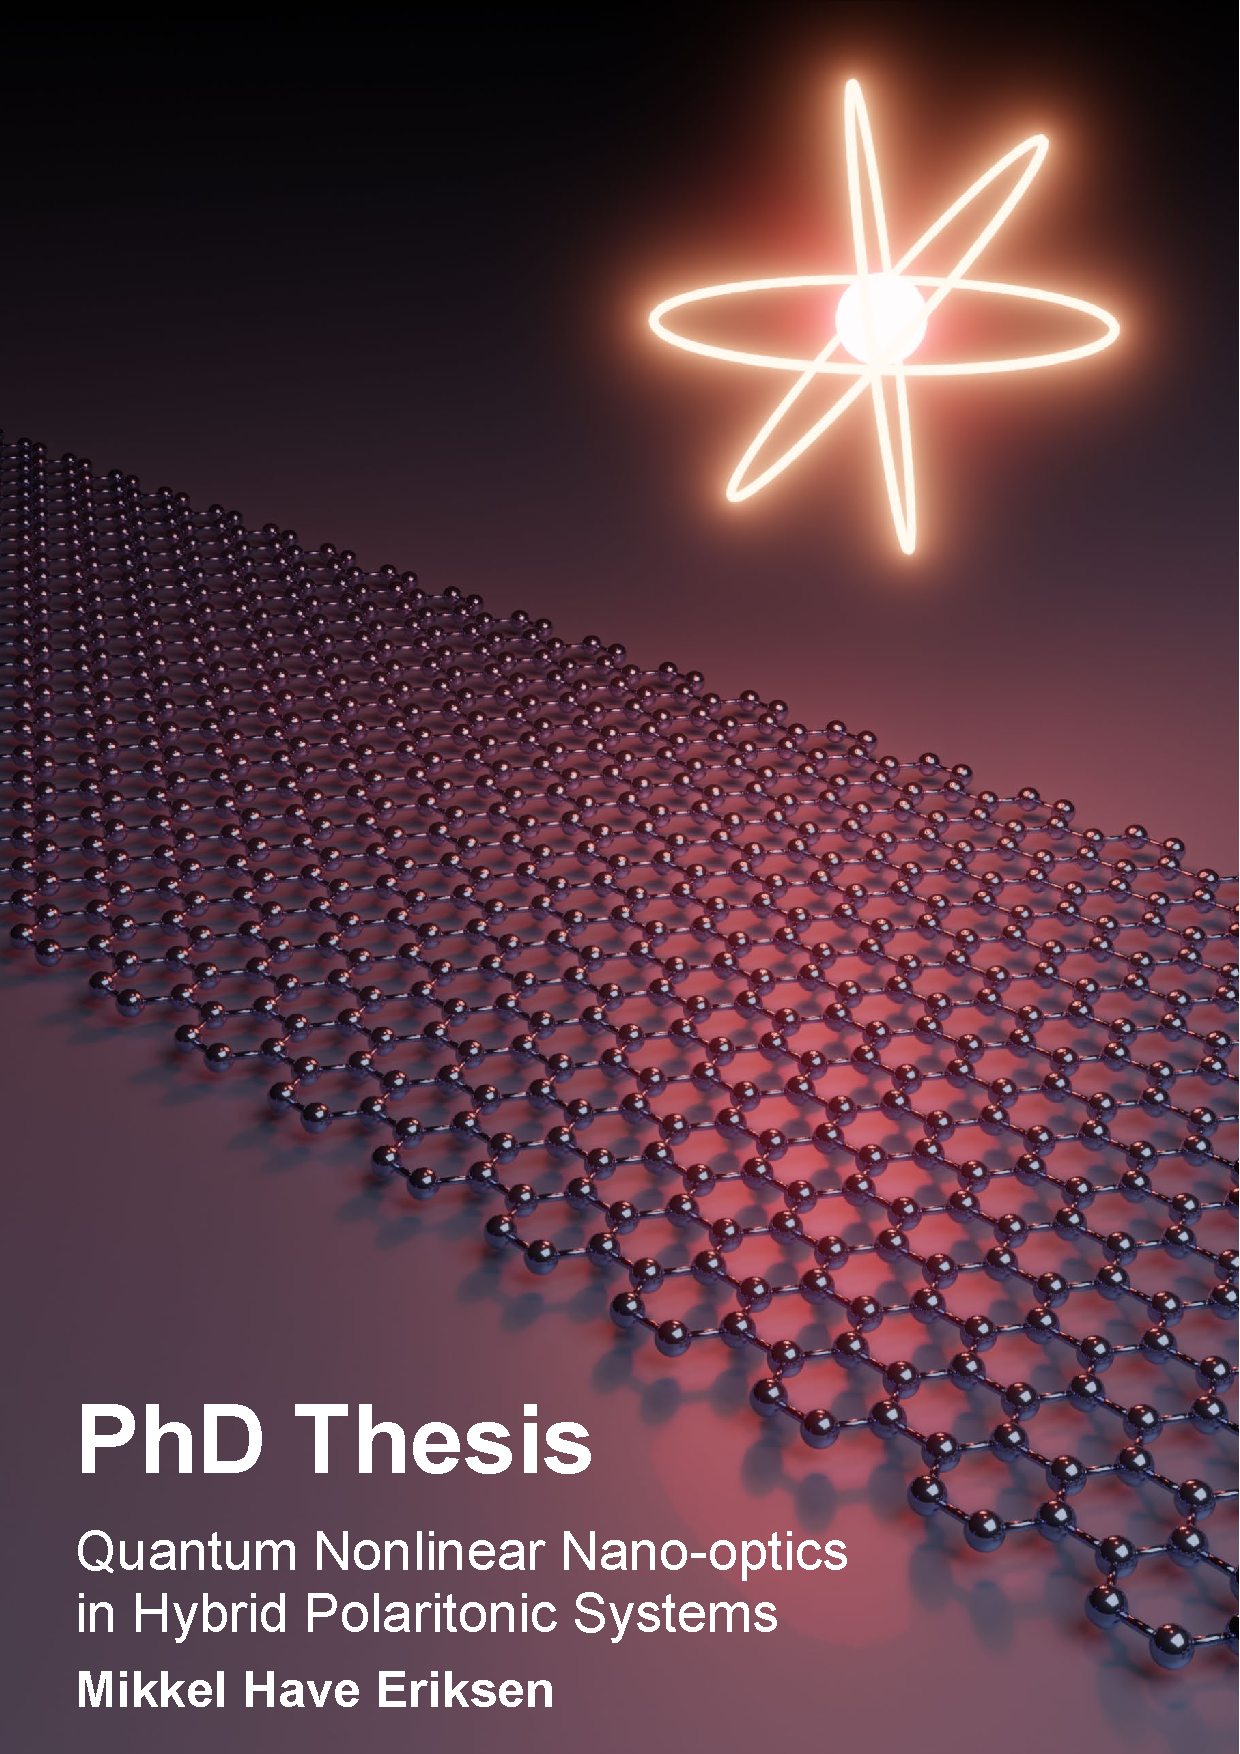
\includegraphics[width=\paperwidth,height=\paperheight,keepaspectratio]{Cover/cover}
    }};
\end{tikzpicture}

\clearpage

{\null\thispagestyle{empty}\newpage} %add blank page

\thispagestyle{empty}
\begin{tikzpicture}[remember picture,overlay]
    \node (fondo) [rectangle]
    at (current page.center)
        {\parbox[b][\paperheight]{\paperwidth}{
        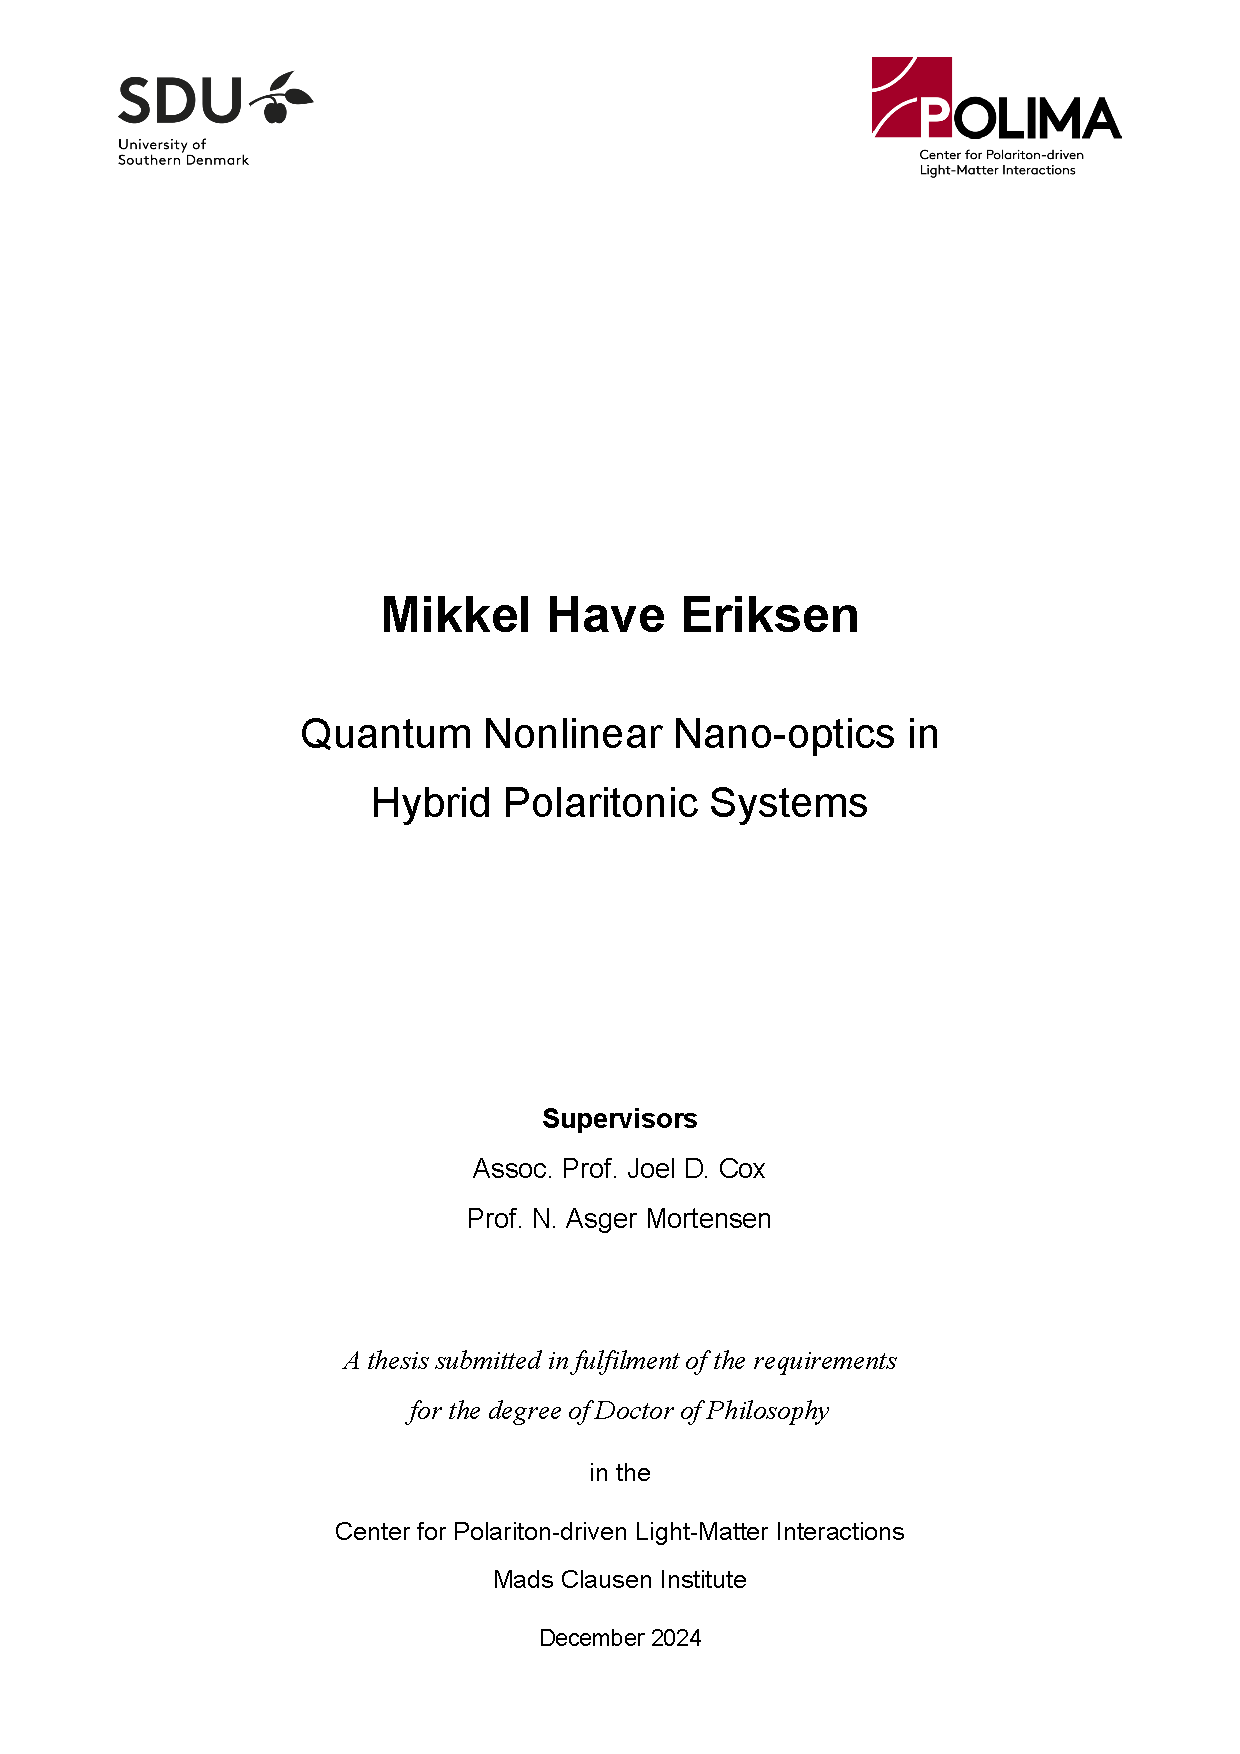
\includegraphics[width=\paperwidth,height=\paperheight,keepaspectratio]{Cover/info_page}
    }};
\end{tikzpicture}

\clearpage

{\null\thispagestyle{empty}\newpage} %add blank page

%%------------------------------------------------------------
%% Print front matter
\texprof{\benchmarktic}
\ntprint{frontmatter}     % The default order is listed below, but can be changed
\texprof{\benchmarktoc}
\texprof{\typeout{TIME process frontmatter=\the\pdfelapsedtime}}
%%------------------------------------------------------------
%% Print main matter
\texprof{\benchmarktic}
\ntthesismainmatter     % The main text — Arabic page numbering
\ntprint{mainmatter}      % The default order is listed below, but can be changed
\texprof{\benchmarktoc}
\texprof{\typeout{TIME process mainmatter=\the\pdfelapsedtime}}
%%------------------------------------------------------------
%% Print back cover and spine
\texprof{\benchmarktic}
\ntprint{backcover}       % Print the back cover, if any!
\texprof{\benchmarktoc}
\texprof{\typeout{TIME process backcover=\the\pdfelapsedtime}}
%%------------------------------------------------------------
\end{document}          % End of document
